\documentclass{article}

% encoding
\usepackage[french]{babel}
\usepackage[T1]{fontenc}
\usepackage[utf8]{inputenc}

%% Bibliography style:
\usepackage{mathptmx}           % Use the Times font.
\usepackage{graphicx}           % Needed for including graphics.
\usepackage{float}              % Better placement of graphics
\usepackage{url}                % Facility for activating URLs.

%% Set the paper size to be A4, with a 2cm margin 
%% all around the page.
\usepackage[a4paper,margin=2cm]{geometry}

% Multicols
\usepackage{multicol}
\usepackage{caption}

%% Natbib is a popular style for formatting references.
\usepackage{natbib}
%% bibpunct sets the punctuation used for formatting citations.
\bibpunct{(}{)}{;}{a}{,}{,}

%% textcomp provides extra control sequences for accessing text symbols:
\usepackage{textcomp}
\newcommand*{\micro}{\textmu}
%% Here, we define the \micro command to print a text "mu".
%% "\newcommand" returns an error if "\micro" is already defined.

%% This is an example of a new macro that I've created to save me
%% having to type \LaTeX each time.  The xspace command provides space
%% after the word LaTeX where appropriate.
\usepackage{xspace}
\providecommand*{\latex}{\LaTeX\xspace}
%% "\providecommand" does nothing if "\latex" is already defined.


% Unicode character in math mode
\usepackage{textcomp}
\usepackage{gensymb}
\usepackage{newunicodechar} 
\newunicodechar{°}{\degree} 


%% Math pagrages
\usepackage{amsmath}
\usepackage{amsfonts}
\usepackage{amssymb}



%----------------------------------------------------------------------------------------
% Code snippets
% ---------------------------------------------------------------------------------------
\usepackage{listings} % Required for inserting code snippets
\usepackage[usenames,dvipsnames]{color} % Required for specifying custom colors and referring to colors by name


\definecolor{DarkGreen}{rgb}{0.0,0.4,0.0} % Comment color
\definecolor{highlight}{RGB}{255,251,204} % Code highlight color

\lstdefinestyle{cpp}{ % Define a style for your code snippet, multiple definitions can be made if, for example, you wish to insert multiple code snippets using different programming languages into one document
language=C++, % Detects keywords, comments, strings, functions, etc for the language specified
backgroundcolor=\color{highlight}, % Set the background color for the snippet - useful for highlighting
basicstyle=\footnotesize\ttfamily, % The default font size and style of the code
breakatwhitespace=false, % If true, only allows line breaks at white space
breaklines=true, % Automatic line breaking (prevents code from protruding outside the box)
captionpos=b, % Sets the caption position: b for bottom; t for top
commentstyle=\usefont{T1}{pcr}{m}{sl}\color{DarkGreen}, % Style of comments within the code - dark green courier font
deletekeywords={}, % If you want to delete any keywords from the current language separate them by commas
%escapeinside={\%}, % This allows you to escape to LaTeX using the character in the bracket
firstnumber=1, % Line numbers begin at line 1
frame=single, % Frame around the code box, value can be: none, leftline, topline, bottomline, lines, single, shadowbox
frameround=tttt, % Rounds the corners of the frame for the top left, top right, bottom left and bottom right positions
keywordstyle=\color{Blue}\bf, % Functions are bold and blue
morekeywords={}, % Add any functions no included by default here separated by commas
numbers=left, % Location of line numbers, can take the values of: none, left, right
numbersep=10pt, % Distance of line numbers from the code box
numberstyle=\tiny\color{Gray}, % Style used for line numbers
rulecolor=\color{black}, % Frame border color
showstringspaces=false, % Don't put marks in string spaces
showtabs=false, % Display tabs in the code as lines
stepnumber=5, % The step distance between line numbers, i.e. how often will lines be numbered
stringstyle=\color{Purple}, % Strings are purple
tabsize=2, % Number of spaces per tab in the code
}

% Create a command to cleanly insert a snippet with the style above anywhere in the document
\newcommand{\insertcode}[2]{\begin{itemize}\item[]\lstinputlisting[caption=#2,label=#1,style=Style1]{#1}\end{itemize}} % The first argument is the script location/filename and the second is a caption for the listing
%----------------------------------------------------------------------------------------


%%%%%%%%%%%%%%%%%%%%%%%%%%%%%%%%%%%%%%%%%%%%%%%%%%%%%%%%%%%%%%%%%%%%%%
%% Start of the document.
%%%%%%%%%%%%%%%%%%%%%%%%%%%%%%%%%%%%%%%%%%%%%%%%%%%%%%%%%%%%%%%%%%%%%%

\begin{document}

\author{Arnaud TANGUY\\
			Jean-Dominique Favreau\\
  University of Polytech'Nice-Sophia}
\date{\today}
\title{Algorithmie Géométrique : Détection de composantes principales}
\maketitle
\begin{abstract}
	Durant ce projet, nous avons exploré des méthodes de détection de composantes principales. La méthode que nous avons sélectionnée est basée sur un accumulateur: la \emph{sphère de Gauss}. Nous avons ensuite exploité les directions prinipales afin de chercher les plans principaux présent dans divers nuages de points.
\end{abstract}

\bigskip

\tableofcontents

\newpage


\section{Sphère de Gauss}
Afin de détecter les directions principales, nous avons choisi de nous intéresser en particulier à un accumulateur: la \emph{sphère de Gauss}.
Le principe est simple: on détermine la normale à chaque point d'un nuage de point, et on accumule la direction de cette normale sur une sphère.

\begin{figure}[H]
    \begin{center}
        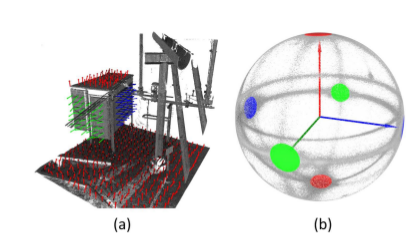
\includegraphics[width=.9\linewidth]{gauss_sphere.png}
    \end{center}
    \caption{Sphère de Gauss telle que présentée dans \protect\citep{Gauss}. (a) Visualisation des normales, (b) Projection des normales sur la sphère de Gauss.}
    \label{fig:gauss_sphere_3D}
\end{figure}

\subsection{Projection Stéréographique}

Nous avons choisi d'accumuler les normales selon une projection stéréographique. 
Cette projection permet de représenter une sphère sur un plan en définissant la position des 
points projetés comme l'intersection de droites passant par les points de la sphère avec un plan.
Dans la suite, on définit les coordonnées par rapport à un repère cartésien $(x,y,z)$ centré en $O$: centre de la sphère de Gauss, définit comme une boule unité centrée en 0.


\begin{figure}[H]
    \begin{center}
        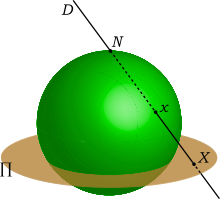
\includegraphics[width=.5\linewidth]{../220px-Stereo.png}
    \end{center}
    \caption{Schéma de la projection stéréographique depuis le point N sur le plan $\Pi$}
    \label{fig:gauss_sphere_schema}
\end{figure}


\begin{itemize}
\item On définit un point $N=\left(\begin{array}{l}0\\ 0\\ \alpha\end{array}\right)$ comme origine de la projection.
\item Le point $x=\left(\begin{array}{l}x_1\\ x_2\\ x_3\end{array}\right)$ coïncide avec les normales, pour peu que celles-ci aient été normalisées au préalable.
\item Le point $X$ représente le point de projection stéréographique sur le plan $\Pi : z=-\beta$\\
On a : $X = \left(\begin{array}{l}0\\ 0\\ \alpha\end{array}\right)+\lambda\left(\begin{array}{l}x_1\\ x_2\\ x_3-\alpha\end{array}\right)$
avec $\lambda = \dfrac{\alpha+\beta}{\alpha-x_3}$
\end{itemize}

En utilisant cette méthode, nous avons généré une projection de la sphère de Gauss en 2 hémisphère. En voici un exemple sur un nuage de point représentant un appartement.

\begin{figure}[H]
\centering
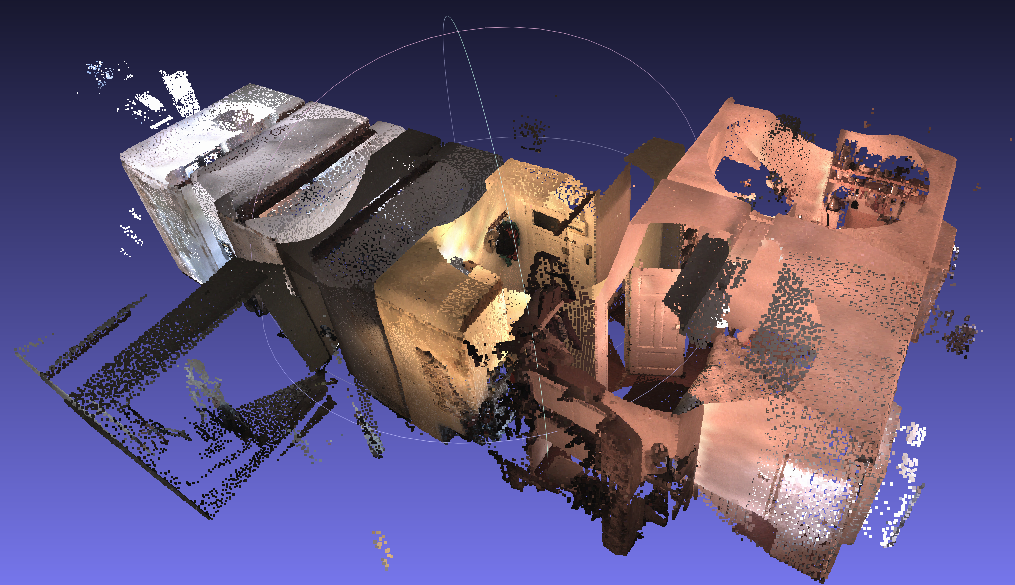
\includegraphics[width=\textwidth]{../2014-02-28-101630_1015x585_scrot.png}
\label{fig:appartement}
\caption{Appartement}

\centering
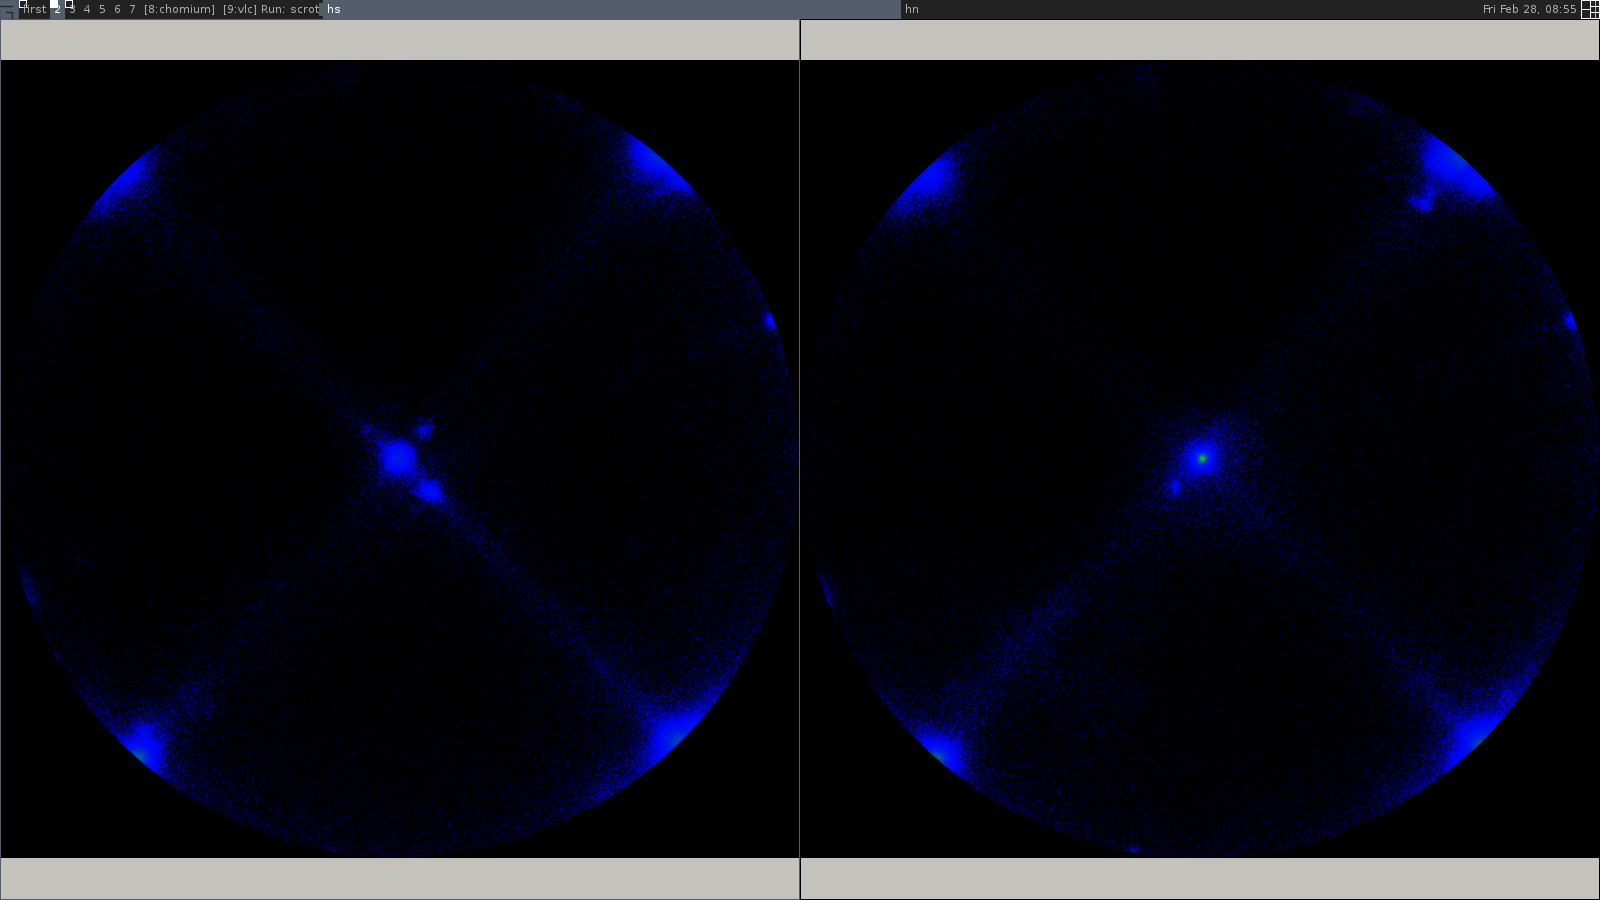
\includegraphics[width=\textwidth]{../2014-02-28-085643_1600x900_scrot.png}
\caption{Sphère de Gauss normalisée, avec $\alpha=1$, $\beta=1000$. La partie gauche représente l'hémisphère sud, la droite l'hémisphère nord.}
\label{fig:gauss_sphere_projection}
\end{figure}

Les zones bleues représentent la position à laquelle les normales ont majoritairement été projetées. On constate nettement que la majorité des normales est concentrée en 6 clusters indépendants: les 4 clusters présent sur le bord de l'image représentent les directions principales des murs verticaux, tandis que la zone centrale représente respectivement le sol (gauche) et le plafond (droite).


Ce type de projection présente de nombreux avantages:
\begin{itemize}
\item La sphère de Gauss est représentée en 2D, permettant ainsi l'utilisation d'algorithme de traitement d'images classiques, tels que le mean-shift.
\item En modifiant les paramètres $\alpha$ et $\beta$ de la projection, on obtient diverses résolution de représentation des normales. On peut alors utiliser ces différents niveaux de résolution afin de rechercher simplement et efficacement de façon hiérarchique les directions principales.
\end{itemize}

Elle présente cependant un avantage majeur: les aires ne sont pas respectées. Il est cependant possible de calculer l'expansion d'aire en fonction de l'angle de projection, et ainsi d'appliquer une distorsion restaurant la notion d'aire.

\subsection{Détection de plans}

La projection stéréographique présente de nombreux avantages, notamment pour la détection de plans. Un plan est idéalement représentable comme un point sur la sphère de Gauss, et donc sur sa projection. En pratique, les normales sont bruitées, et forment un blob par direction principale (voir \ref{fig:gauss_sphere_projection}).

Afin d'obtenir la normale idéale représentant la direction principale de chaque cluster, il nous faut:
\begin{itemize}
\item Extraire les différents blobs de l'image
\item Déterminer la normale optimale dans le cluster.On peut utiliser un algorithme tel que \emph{mean shift} afin de déterminer le centre du cluster.
\end{itemize}

Pour cela, on peut commencer à travailler sur une sphère de Gauss à faible résolution ($\alpha$ élevé et $\beta$ faible).

\begin{figure}[H]
\centering
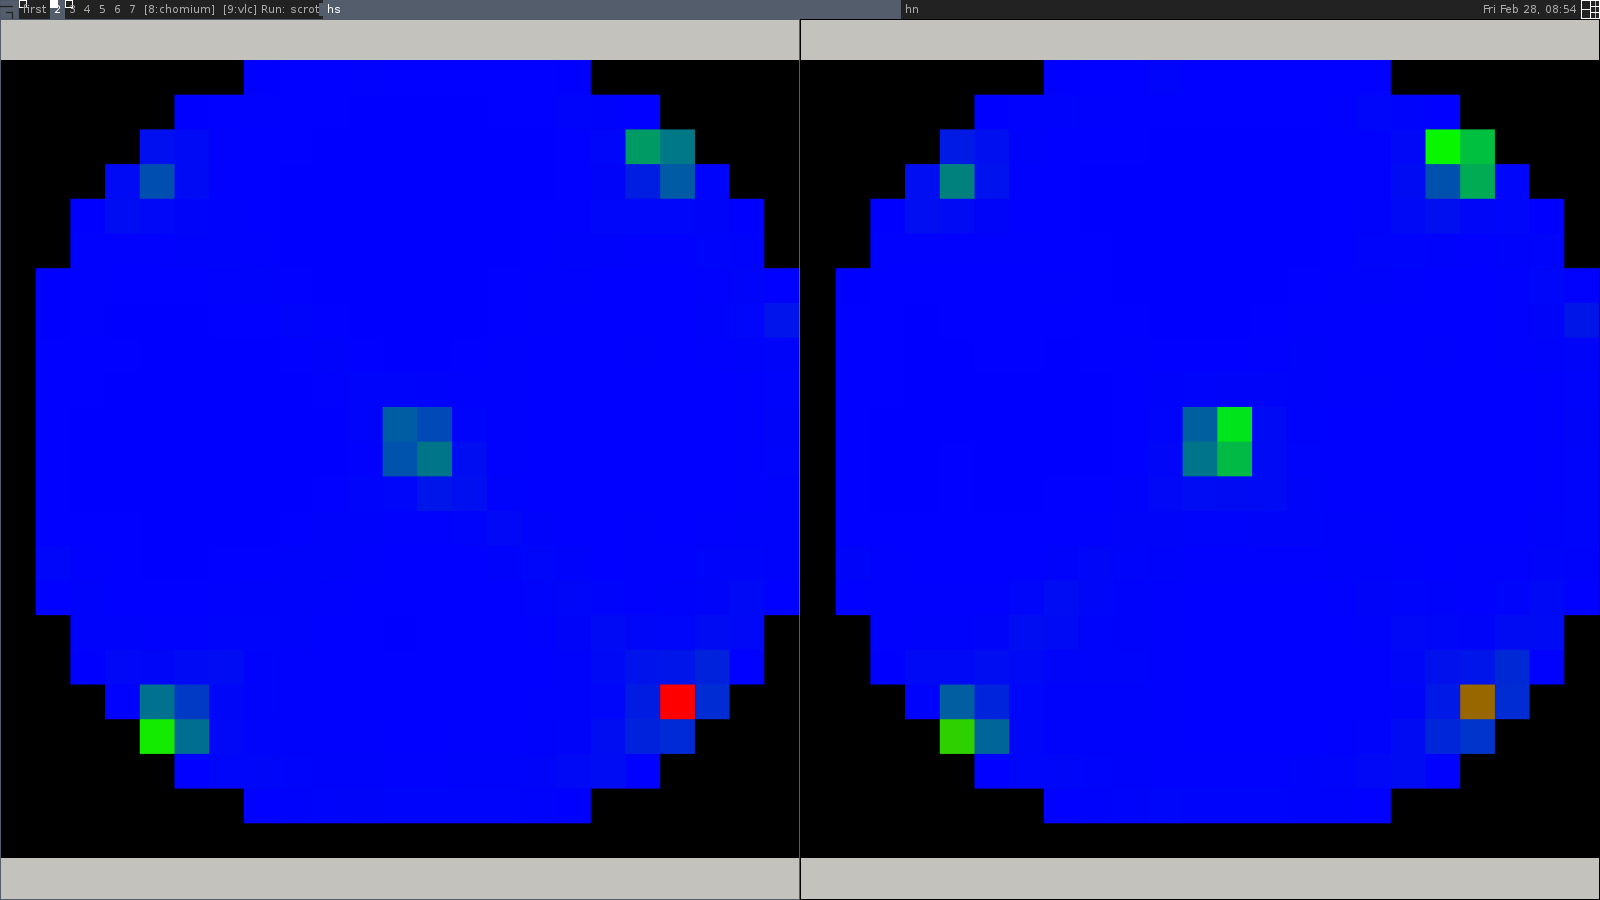
\includegraphics[width=\textwidth]{../2014-02-28-085518_1600x900_scrot.png}
\caption{Sphère de Gauss de l'appartement avec $\alpha=1$ et $\beta=10$}
\label{fig:sphere_gauss_low_res}
\end{figure}

Comme on peut le voir en comparant la figure \ref{fig:gauss_sphere_projection} et \ref{fig:sphere_gauss_low_res}, il est aisé de trouver les clusters de façon hiérarchique. On peut par exemple choisir de chercher le pixel ayant l'intensité maximale sur l'image basse résolution (figure \ref{fig:sphere_gauss_low_res}). Ce pixel correspondra à un cluster sur une image à résolution (figure \ref{fig:gauss_sphere_projection}) plus élevée. En effectuant un mean-shift sur le cluster sélectionné dans l'image haute résolution, il est alors possible de trouver la normale représentant au mieux le cluster.

\begin{figure}[H]
\centering
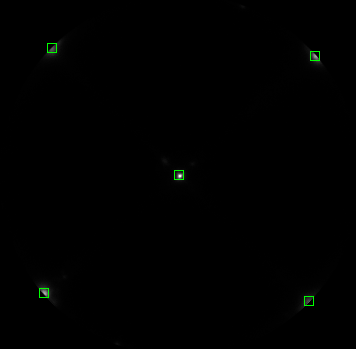
\includegraphics[width=.5\columnwidth]{../blob.png}
\caption{Détection des clusters principaux dans la sphère de Gauss}
\label{fig:clusters_gauss}
\end{figure}


\subsection{Détection de cylindres}
Les formes cylindriques accumulent leur normales selon un cercle sur la sphère de Gauss. La direction principale du cylindre est orthogonale au plan de support de ce cercle.

Dans notre espace de représentation projeté, un cylindre résulte en
\begin{description}
\item[Un cercle] Si la direction principale est orientée selon $\pm \left(\begin{array}{l}0\\1\\0\end{array}\right)$
\item[Une ellipse] dans tous les autres cas.
\end{description}

Voici un exemple de résultat obtenu sur un nuage de point de l'Église St. Jean, ayant une forme cylindrique.


\begin{multicols}{2}
\begin{figure}[H]
\centering
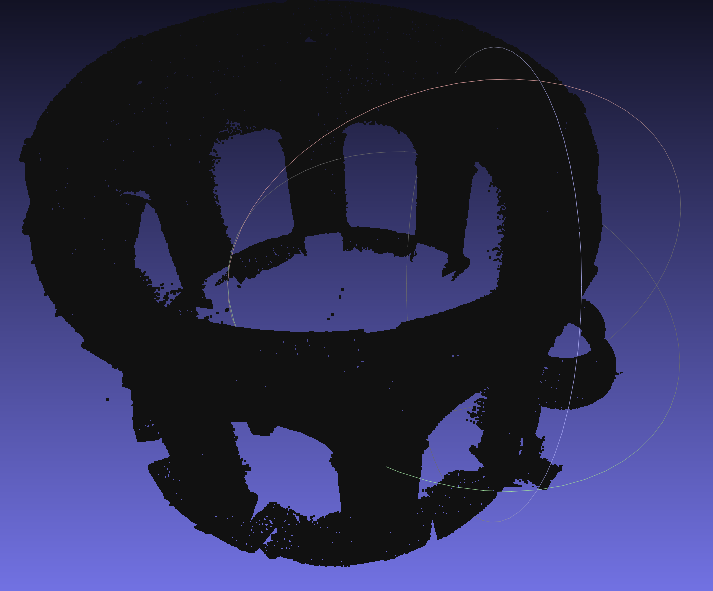
\includegraphics[width=\columnwidth]{../2014-02-28-102010_713x591_scrot.png}
\caption{église $S^t$ Jean}
\end{figure}

\columnbreak

\begin{figure}[H]
\centering
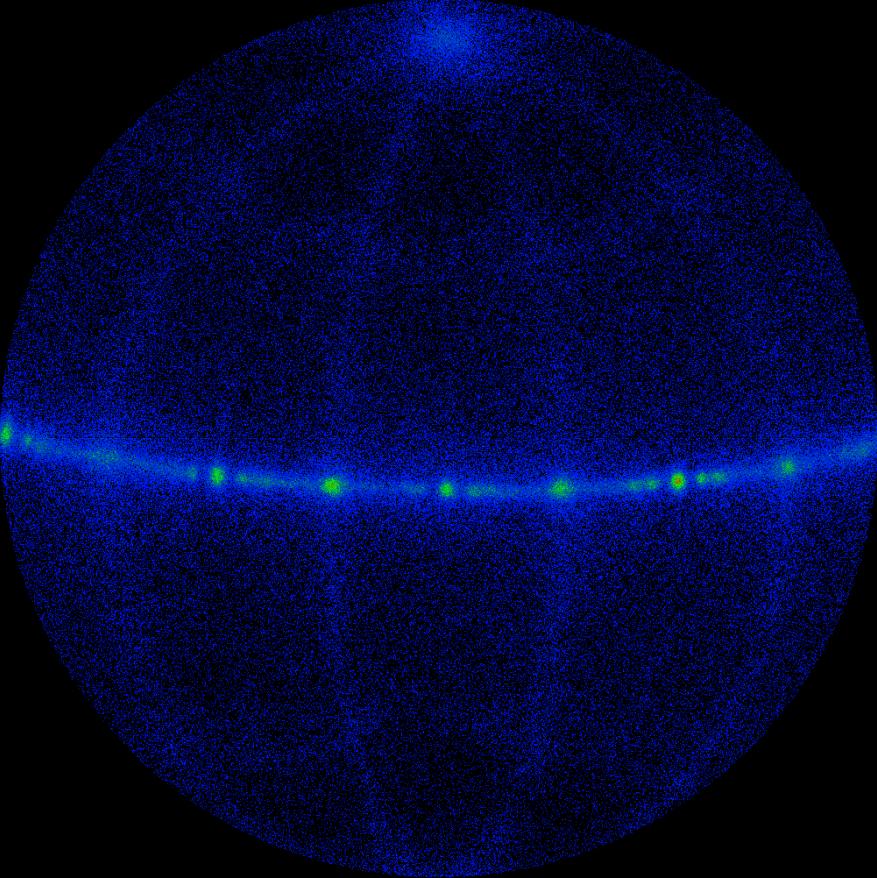
\includegraphics[width=\columnwidth]{../gauss_st_jean.png}
\caption{Sphère de Gauss de l'église, avec $\alpha=1$ et $\beta=1000$}
\end{figure}
\end{multicols}

L'arc bleu clair horizontal sur la sphère de gauss représente la direction des normales horizontales de l'église, c'est à dire toute la façade circulaire. Chaque point sur cet arc correspond à une colonne. Les arcs de cercle verticaux représentent la courbure des arches.

Cet espace de représentation est donc loin d'être adapté à la détection des cylindres.









\section{Reconstruction de plans}

Une fois les directions principales des plans obtenues, il s'agit de trouver les plans dans le nuage de point. Il peut y avoir plusieurs plans à des profondeurs différentes selon une direction de normale. Pour cela, on a étudié la distribution des points selon la normale. L'idée est que les points représentant un même plan seront tous plus ou moins à la même distance de l'origine dans la direction de la normale.

\begin{figure}[H]
\centering
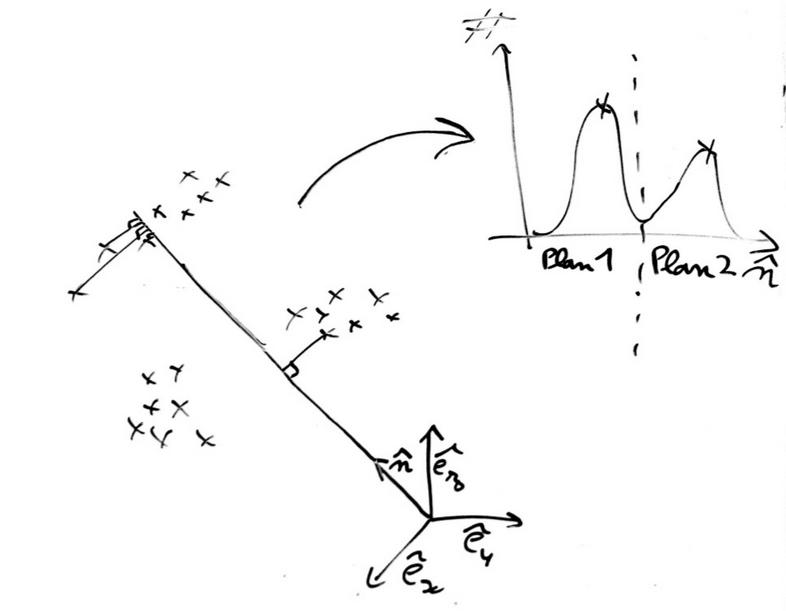
\includegraphics[width=.7\textwidth]{../normal_to_hist.png}
\caption{Distribution des plans selon la normale. On représente le nombre de points en fonction de la distance par rapport à l'origine dans la direction de la normale.}
\end{figure}


Sur la figure ci-dessus, il est clairement visible que les points sont répartis selon 2 plans. Afin de les détecter, on seuille l'histogramme et cherche le maximum de chacun des pics. Sur des nuages de points réels, l'histogramme est bien sur bien moins régulier.

\begin{figure}[H]
\centering
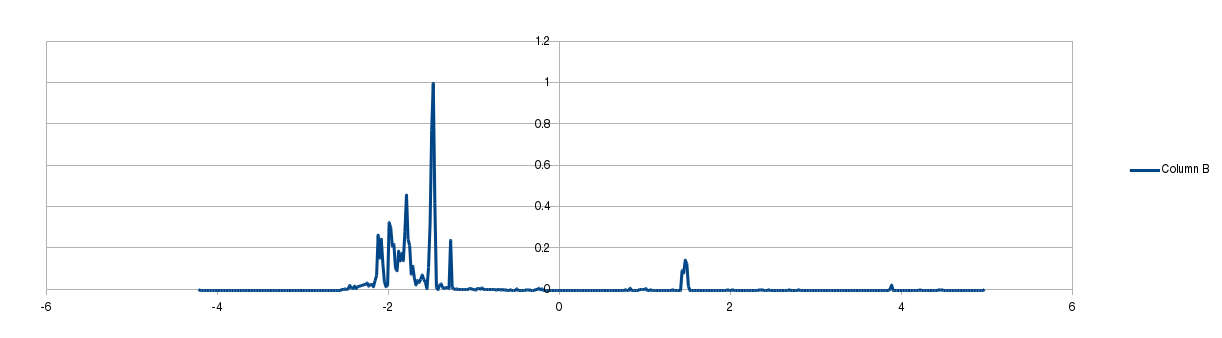
\includegraphics[width=\columnwidth]{../distribution_along_normal.png}
\caption{Histogramme dans une direction principale de l'appartement (normale horizontale correspondant aux murs). }
\end{figure}
\begin{figure}[H]
\centering
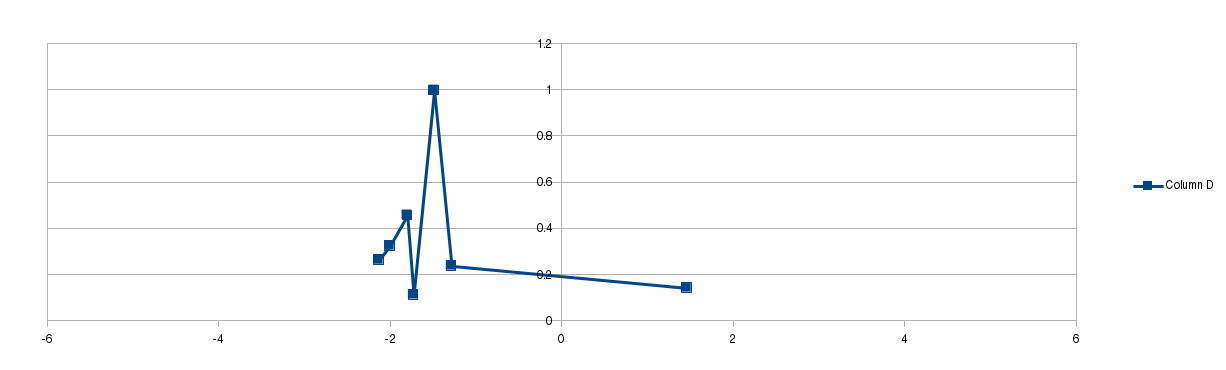
\includegraphics[width=\columnwidth]{../distribution_along_normal_max.png}
\caption{Histogramme seuillé: les points représentent plans détecté (leur abscisse correspond à la position en mètres depuis l'origine du plan).}
\end{figure}


Afin d'améliorer la détection de la position des plans, il serait intéressant d'imposer une distance minimale entre 2 plans. Considérant que le bruit dans les données est assimilable à 
du bruit Gaussien, on pourrait également chercher les distributions gaussiennes représentant au mieux l'histogramme, et déterminer la position des plans en fonction de la moyenne et variance de ces distributions.

Les plans sont ensuite reconstruit de façon très approximative, en considérant seulement le plus petit rectangle englobant toutes les données classifiées comme appartenant à une profondeur de plans. Cette méthode n'est bien sur par robuste aux outliers, et ne permet pas de distinguer différents plans à une même profondeur. Afin d'obtenir un meilleur résultat, il serait intéressant d'utiliser une combinaison de RANSAC et K-Means afin de clusteriser les plans 
et reconstruire autant de plans qu'il y a de clusters trouvés sans tenir compte des outliers.


\section{Résultats}

\begin{multicols}{2}
\begin{figure}[H]
\centering
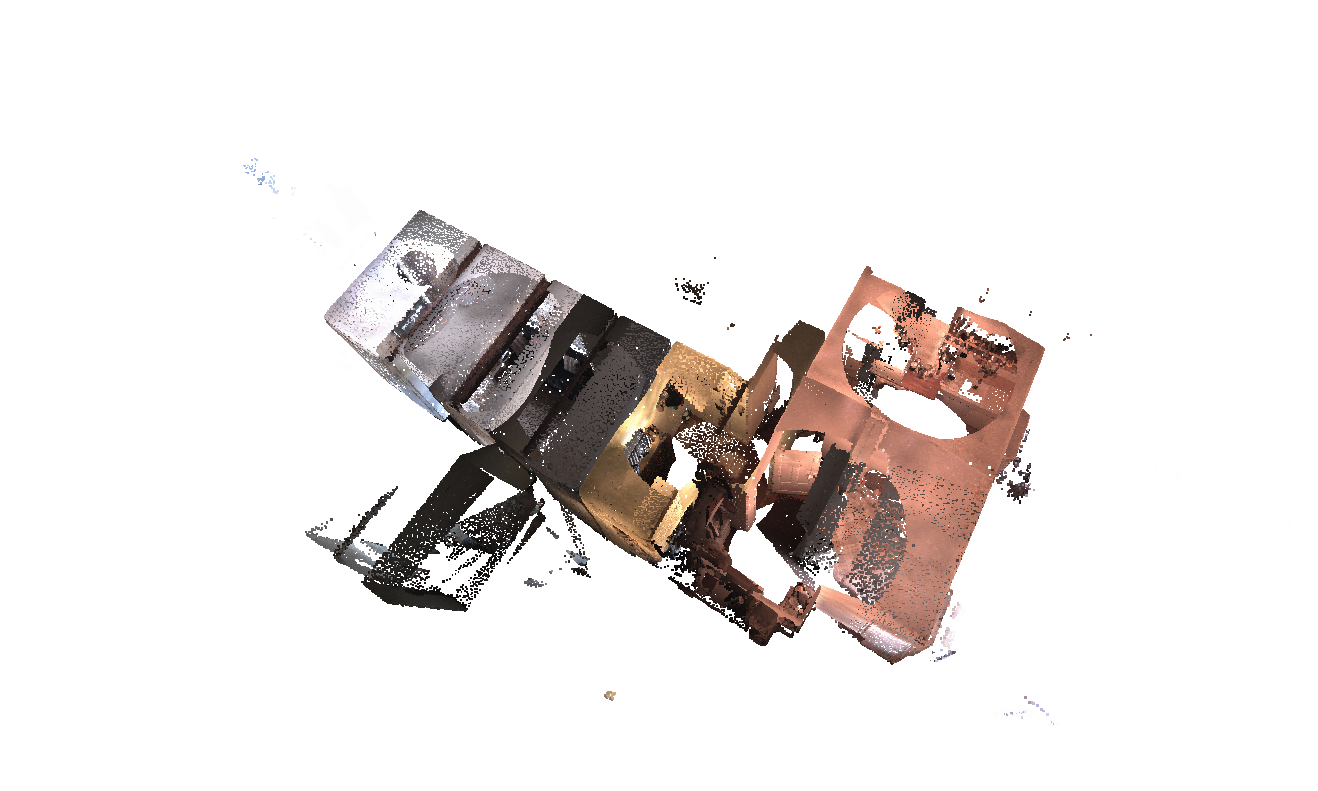
\includegraphics[width=1.3\columnwidth]{../appart01.png}
\caption{Appartement: nuage de points de référence}
\end{figure}

\columnbreak
\begin{figure}[H]
\centering
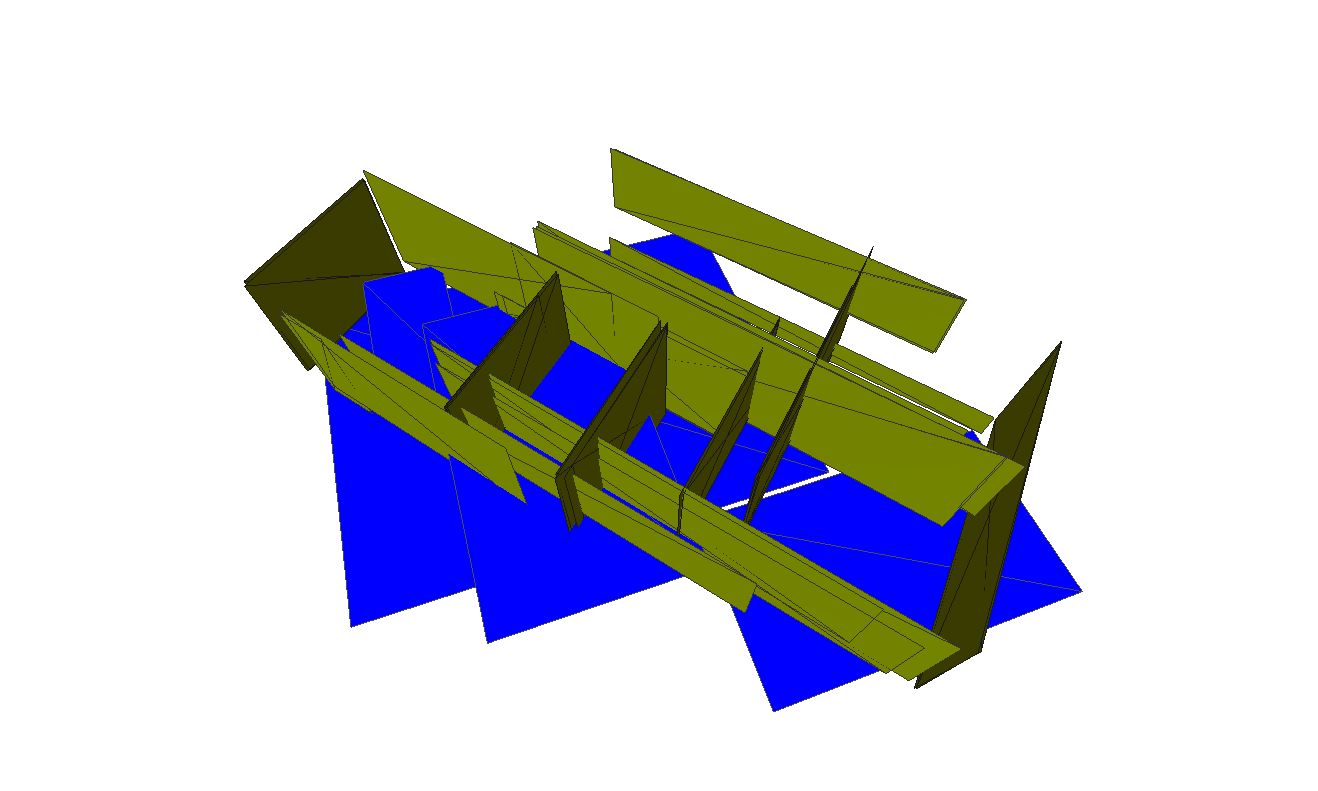
\includegraphics[width=1.3\columnwidth]{../appart04.png}
\caption{Plans reconstruits avec $\beta$ élevé.}
\end{figure}

\end{multicols}


\begin{figure}[H]
\centering
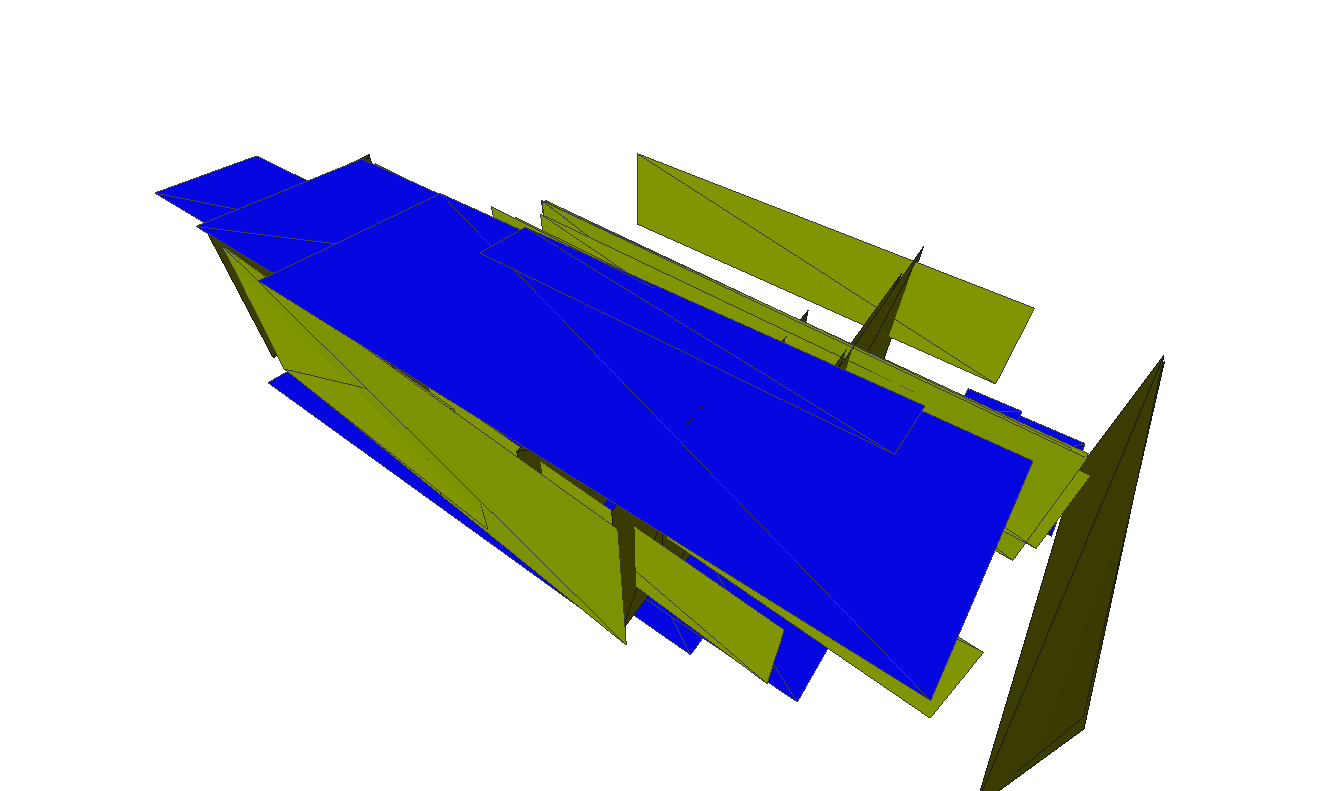
\includegraphics[width=\columnwidth]{../appart06.png}
\caption{Plans reconstruits, avec $\beta$ plus faible. On remarque que cette fois-ci le toit a été détecté. Cela est du au fait que les normales représentant le toit sont realivement bruitée, et diminuer la résolution de la projection induit un phénomène de clustering concentrant toutes les normales sur une plus petite zone.}
\end{figure}


\begin{figure}[H]
\centering
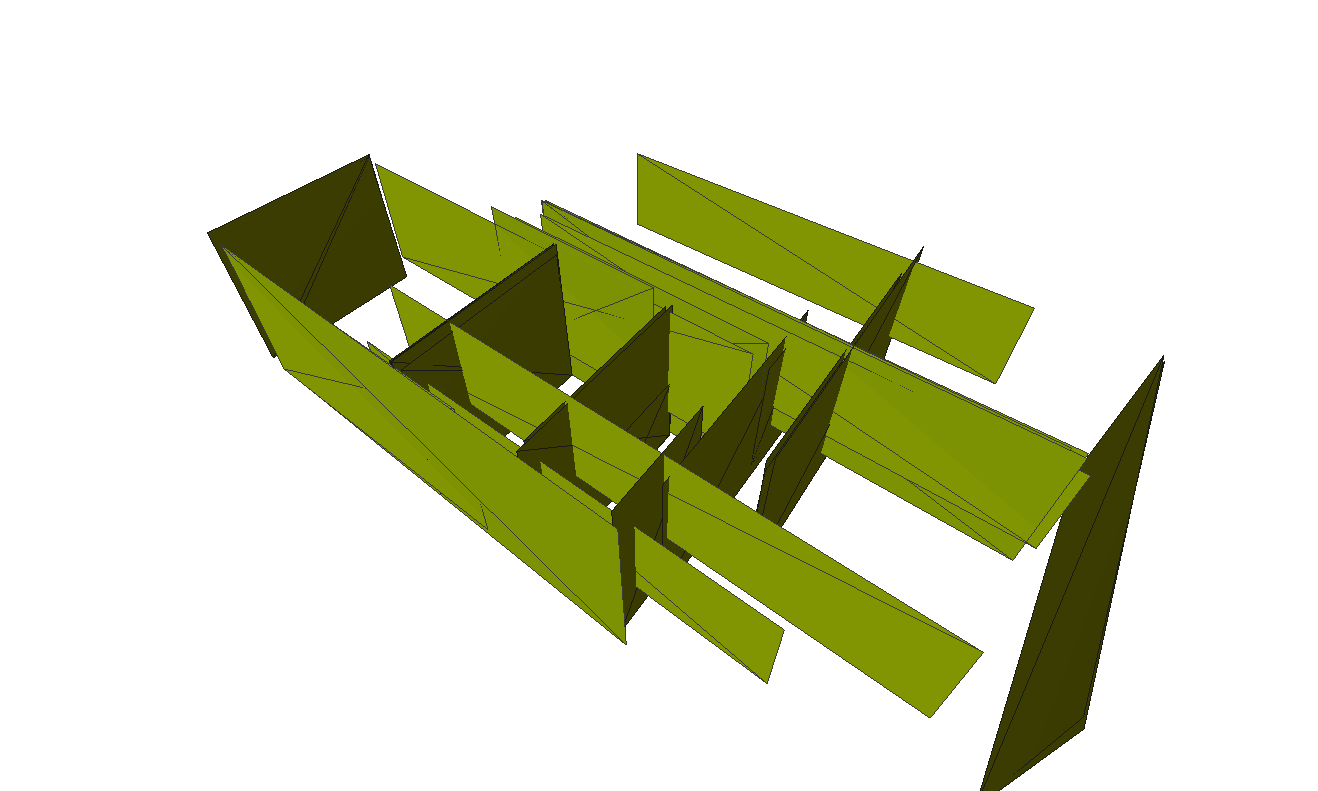
\includegraphics[width=\columnwidth]{../appart05.png}
\caption{Si l'on enlève le toit de la figure précédente, on peu voir les plans reconstruits à l'intérieur de l'appartement. On constante que diminuer la résolution de la sphère de Gauss a introduit des erreurs d'orientation de normales. Par exemple, le plan le plus à droite est très mal orienté.}
\end{figure}

\begin{figure}[H]
\centering
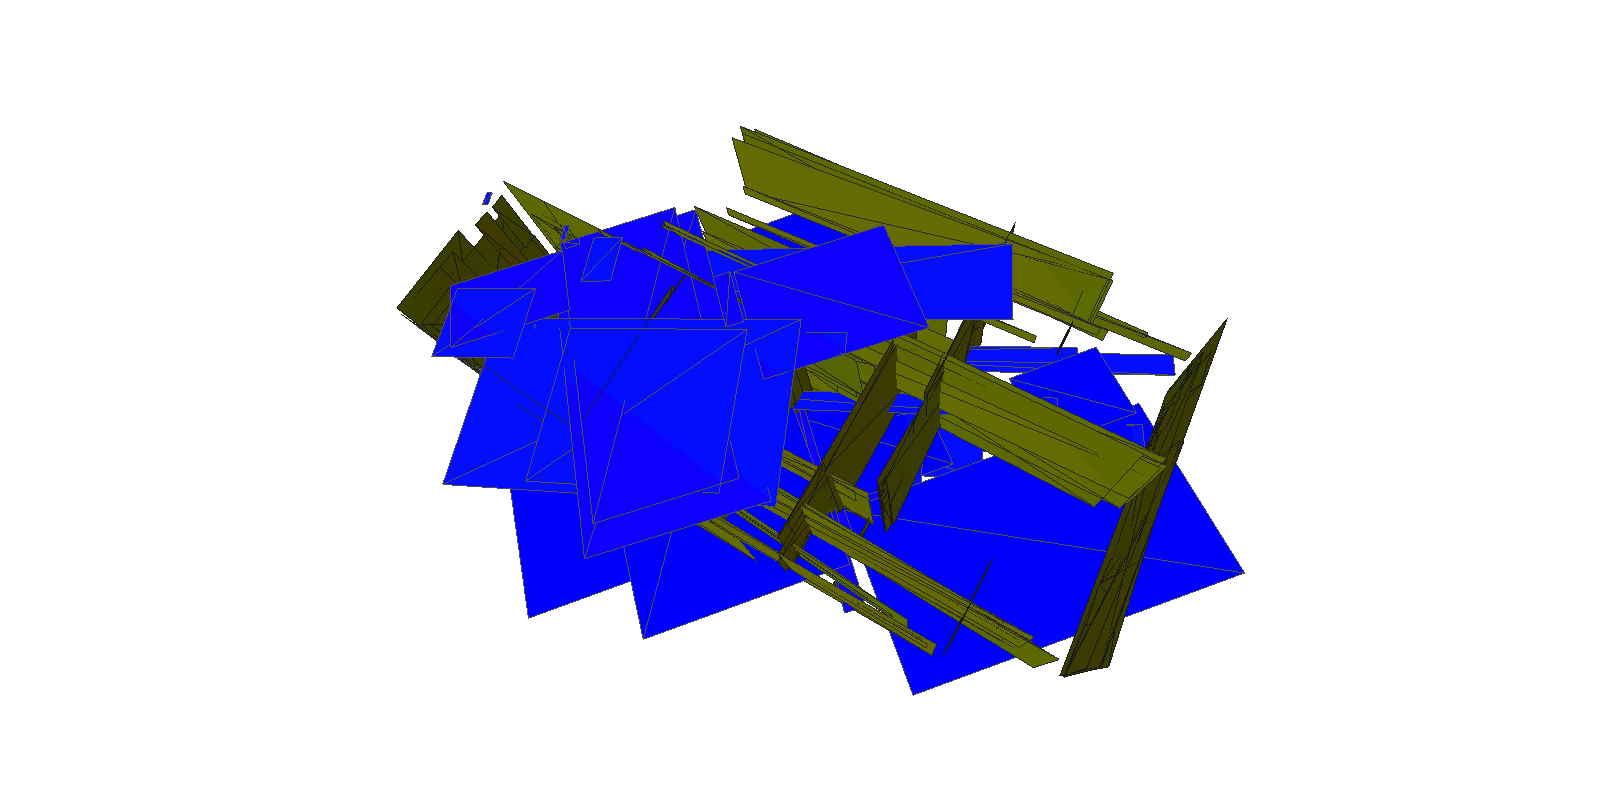
\includegraphics[width=\columnwidth]{../appart00.png}
\caption{Les erreurs d'orientations sont généralement compensée en prenant le centre d'un cluster comme orientation de normale. Cette figure représente le résultat obtenu lorsque le clustering n'est pas effectué et que la direction des normales est directement prise comme étant le maximum de chaque cluster.}
\end{figure}


\section{Détails d'implémentation}
\subsection{Sphère de Gauss sur GPU}
La projection stéréographique des normales sur la sphère de Gauss est hautement parallélisable. En effet, la sphère de gauss étant un simple accumulateur, la projection de toutes les normales peut être implémentée en parallèle. 

Cependant, beaucoup de normales doivent être accumulées au même endroit, entrainant des délais d'écriture du fait de l'atomicité de l'accumulation (il n'est pas possible d'accumuler plusieurs normales au même endroit en même temps, cette opération doit être effectuée séquentiellement). Ce problème peut être fortement allégé en prenant les normales dans un ordre aléatoire, réduisant ainsi le nombre de normales devant être simultanément accumulées au même endroit.

Voici le \emph{kernel} OpenCL responsable de la projection

\begin{lstlisting}[language=c,breaklines=true]
void kernel gauss_sphere(volatile global float4* normal, global int* north_hemisphere, global int* south_hemisphere, const float alpha_g, const float beta_g)
{
    private const float beta = beta_g;
    private const float alpha = alpha_g; 
    private const int rows = 2*(1+(int)ceil(beta/alpha)) + 1;
    
    private int index = get_global_id(0);
    private float tmp;
    private int2 coord;
    private float4 n = normal[index];
    // Compute projection for the south hemisphere
    if(n.z<0) {
        tmp = (beta+alpha)/(alpha-n.z);
        coord = convert_int2((float2)(floor(tmp*n.xy)))+ (int2)(rows/2, rows/2);
        private int tex = coord.y * rows + coord.x;
        // Atomic operation to increment the value for the current normal.
        // This ensures that no other normal is currently being accumulated at this position.
        atomic_inc(&south_hemisphere[tex]);
    } 
    // North hemisphere
    else {
        tmp = (beta+alpha)/(alpha+n.z);
        coord = convert_int2((float2)(floor(tmp*n.xy))) + (int2)(rows/2, rows/2);
        private int tex = coord.y * rows + coord.x;
        atomic_inc(&north_hemisphere[tex]);
    }
}
\end{lstlisting}


\section{Conclusion}
La méthode de détection de composante principales basée sur la sphère de Gauss est très prometteuse. Elle est très efficace et performante dans le cadre de plans car ceux-ci projettent énormément de normales au même endroit. Elle n'est cependant pas limitée aux plans, et peut prendre en compte bien d'autres composantes, telle que cylindres, cônes, sphères\ldots.

Afin d'améliorer le travail présenté ici, les articles suivants fournissent des techniques utiles: \citep{Gauss}, \citep{3DReconstructionlod} et \citep{li_globFit_sigg11}



%%%%%%%%%%%%%%%%%%%%%%%%%%%%%%%%%%%%%%%%%%%%%%%%%%%%%%%%%%%%%%%%%%%%%%
%% Finally we specify the format required for our references and the
%% name of the bibtex file where our references should be taken from.
%%%%%%%%%%%%%%%%%%%%%%%%%%%%%%%%%%%%%%%%%%%%%%%%%%%%%%%%%%%%%%%%%%%%%%
\pagebreak
\bibliographystyle{plainnat}
\bibliography{rapport}

\end{document}